%%
%% This is file `sample-sigconf.tex',
%% generated with the docstrip utility.
%%
%% The original source files were:
%%
%% samples.dtx  (with options: `sigconf')
%%
%% IMPORTANT NOTICE:
%%
%% For the copyright see the source file.
%%
%% Any modified versions of this file must be renamed
%% with new filenames distinct from sample-sigconf.tex.
%%
%% For distribution of the original source see the terms
%% for copying and modification in the file samples.dtx.
%%
%% This generated file may be distributed as long as the
%% original source files, as listed above, are part of the
%% same distribution. (The sources need not necessarily be
%% in the same archive or directory.)
%%
%% The first command in your LaTeX source must be the \documentclass command.
\documentclass[sigconf,screen]{acmart}

\settopmatter{printfolios=true}

\usepackage{hyperref}


\providecommand{\tightlist}{%
  \setlength{\itemsep}{0pt}\setlength{\parskip}{0pt}}

%%
%% \BibTeX command to typeset BibTeX logo in the docs
\AtBeginDocument{%
  \providecommand\BibTeX{{%
    \normalfont B\kern-0.5em{\scshape i\kern-0.25em b}\kern-0.8em\TeX}}}

%% Rights management information.  This information is sent to you
%% when you complete the rights form.  These commands have SAMPLE
%% values in them; it is your responsibility as an author to replace
%% the commands and values with those provided to you when you
%% complete the rights form.


%%
%% Submission ID.
%% Use this when submitting an article to a sponsored event. You'll
%% receive a unique submission ID from the organizers
%% of the event, and this ID should be used as the parameter to this command.
%%\acmSubmissionID{123-A56-BU3}

%%
%% The majority of ACM publications use numbered citations and
%% references.  The command \citestyle{authoryear} switches to the
%% "author year" style.
%%
%% If you are preparing content for an event
%% sponsored by ACM SIGGRAPH, you must use the "author year" style of
%% citations and references.
%% Uncommenting
%% the next command will enable that style.
%%\citestyle{acmauthoryear}

%%
%% end of the preamble, start of the body of the document source.
\begin{document}

%%
%% The "title" command has an optional parameter,
%% allowing the author to define a "short title" to be used in page headers.
\title{Web Voyager: Lightweight Exploration Of Semi-Structured Website
Data}

%%
%% The "author" command and its associated commands are used to define
%% the authors and their affiliations.
%% Of note is the shared affiliation of the first two authors, and the
%% "authornote" and "authornotemark" commands
%% used to denote shared contribution to the research.

\author{Kapaya Katongo}
\affiliation{%
  \institution{MIT CSAIL}
  \city{Cambridge, MA}
  \country{USA}
}
\email{kkatongo@mit.edu}

\author{Geoffrey Litt}
\affiliation{%
  \institution{MIT CSAIL}
  \city{Cambridge, MA}
  \country{USA}
}
\email{glitt@mit.edu}

\author{Daniel Jackson}
\affiliation{%
  \institution{MIT CSAIL}
  \city{Cambridge, MA}
  \country{USA}
}
\email{dnj@csail.mit.edu}

%%
%% By default, the full list of authors will be used in the page
%% headers. Often, this list is too long, and will overlap
%% other information printed in the page headers. This command allows
%% the author to define a more concise list
%% of authors' names for this purpose.
% \renewcommand{\shortauthors}{Trovato and Tobin, et al.}

%%
%% The abstract is a short summary of the work to be presented in the
%% article.
\begin{abstract}
  Websites are awash with semi-structured data that is ripe for
  exploration but there are two significant barriers to this: accessing
  the data and visualizing the data. Accessing the data requires
  knowledge of web scraping because the data is often not available in a
  portable format such as JSON or CSV or is only available behind an API
  which requires programming expertise to use. Visualizing the data
  requires knowledge of visualization specification formats or
  languages.

  In this paper, we present an interaction model for lightweight
  exploration of semi-structured website data that does not require
  knowledge of web scraping or data visualization formats and languages.
  Our key idea is to combine web scraping via
  programming-by-demonstration with visualization recommendation: users
  scrape data from a website via mouse clicks and get visualization
  recommendations based on the scraped data. Unlike existing solutions,
  our web scraping approach supports accessing a wide variety of
  semi-structured website data and our visualization approach is neither
  limited to predefined visualizations nor does it require knowledge of
  data visualization.

  To illustrate the proposed model, we have implemented a Chrome browser
  extension called Web Voyager. Through case studies, we show how our
  model can be used to explore data on real-world websites in order to
  characterize the capabilities and limitations of the approach.
\end{abstract}

%%
%% The code below is generated by the tool at http://dl.acm.org/ccs.cfm.
%% Please copy and paste the code instead of the example below.
%%
%% From HERE
\begin{CCSXML}
<ccs2012>
   <concept>
       <concept_id>10003120.10003121.10003124.10010868</concept_id>
       <concept_desc>Human-centered computing~Web-based interaction</concept_desc>
       <concept_significance>500</concept_significance>
       </concept>
   <concept>
       <concept_id>10011007.10011006.10011066.10011069</concept_id>
       <concept_desc>Software and its engineering~Integrated and visual development environments</concept_desc>
       <concept_significance>500</concept_significance>
       </concept>
 </ccs2012>
\end{CCSXML}

\ccsdesc[500]{Human-centered computing~Web-based interaction}
\ccsdesc[500]{Software and its engineering~Integrated and visual development environments}
% To HERE

%%
%% Keywords. The author(s) should pick words that accurately describe
%% the work being presented. Separate the keywords with commas.
\keywords{data visualization, end-user web scraping}

%% A "teaser" image appears between the author and affiliation
%% information and the body of the document, and typically spans the
%% page.
%\begin{teaserfigure}
%  \includegraphics[width=\textwidth]{sampleteaser}
%  \caption{Seattle Mariners at Spring Training, 2010.}
%  \Description{Enjoying the baseball game from the third-base
%  seats. Ichiro Suzuki preparing to bat.}
%  \label{fig:teaser}
%\end{teaserfigure}

%%
%% This command processes the author and affiliation and title
%% information and builds the first part of the formatted document.
\maketitle

\hypertarget{sec:introduction}{%
\section{Introduction}\label{sec:introduction}}

Many websites contain collections of semi-structured data that are ripe
for exploration. This data ranges from job postings on websites like
LinkedIn to user reviews on websites like Yelp. Visualization is a
common way to explore data but to visualize data, it needs to be
accessible in a format suitable for computation. Most website data is
either not available in a portable format such as JSON or CSV or is only
available via an Application Programming Interface (API) which requires
programming expertise to setup. Even with the data in hand, visualizing
it requires knowledge of data visualization specification formats and
languages. Both of these, that is data access and knowledge of data
visualization, can be significant barriers to exploring website data.

Prior research has resulted in tools like Vispedia \citep{chan2008},
Reform \citep{toomim2009} and DS.js \citep{zhang2017} which have
developed solutions to some aspects of the two barriers. Vispedia
automatically accesses website data via web scraping and allows users to
visualize it using a predefined list of visualizations. However, it only
works on Wikipedia. Reform allows users to access website data via
programming-by-demonstration (PBD) based web scraping and feed it into a
predefined visualization widget created by a programmer. While the
visualization widgets are not restricted to any given website, they
require the exact data prescribed by their authors. This means that in
order to visualize data on a website, a programmer must have created a
visualization widget that accepts that type of data. DS.js comes closest
to breaking down the two barriers. It automatically accesses website
data via web scraping and provides a programming environment to analyze
and visualize the scraped data. However, only website data in HTML table
elements can be accessed which does not cover the wide variety of
available semi-structured data on websites. Furthermore, users require
knowledge of programming and data visualization in order to use the
provided programming environment to explore the data.

In this paper, we present an interaction model for lightweight
exploration of semi-structured website data right in the context of the
website. Our key idea is to combine web scraping via PBD with
visualization recommendation: users scrape data from a website via mouse
clicks and get visualization recommendations based on the scraped data.
No knowledge of web scraping or data visualization specification formats
and languages is required! Unlike existing solutions, our web scraping
approach supports accessing a wide variety of semi-structured website
data \emph{and} our visualization approach is neither limited to
predefined visualizations nor does it require knowledge of data
visualization.

\begin{figure*}
  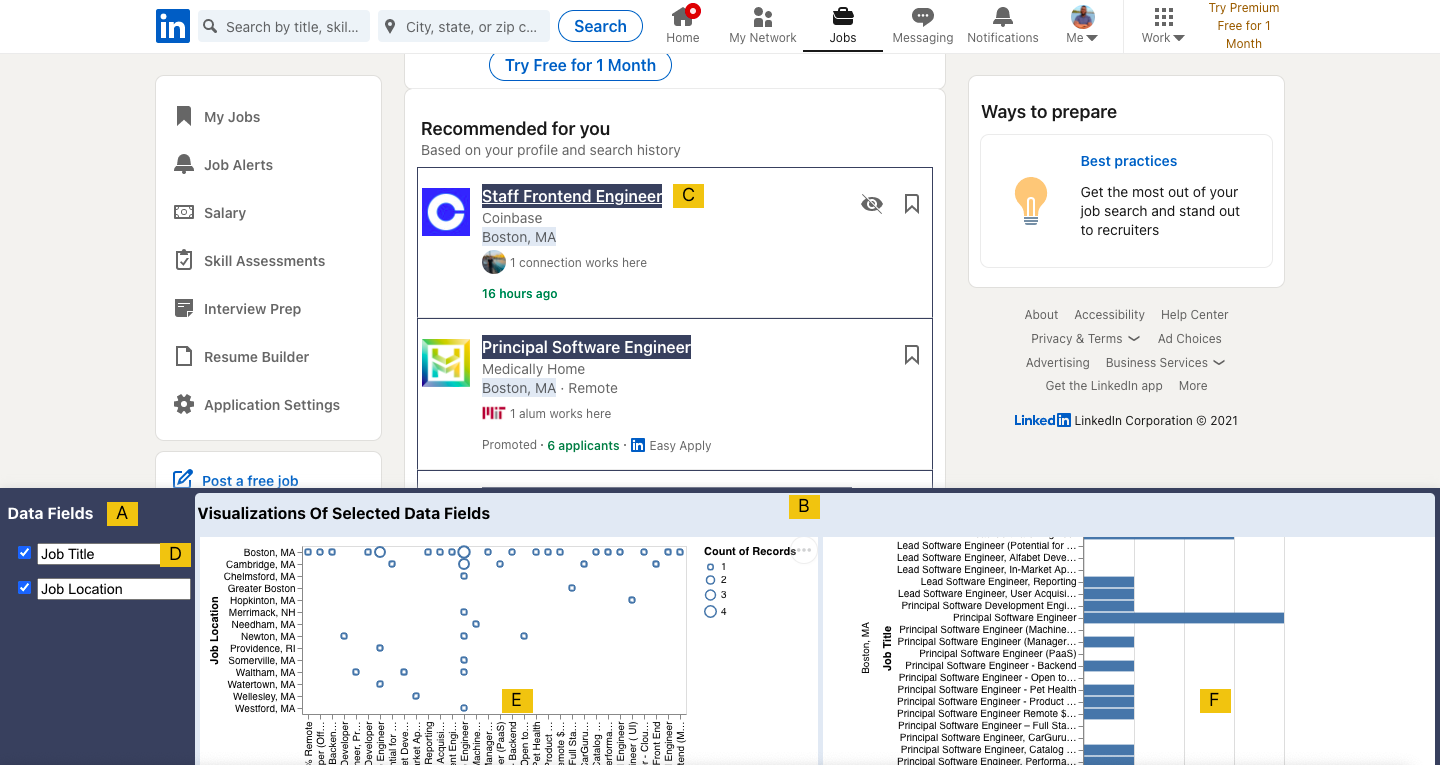
\includegraphics[width=\textwidth]{media/example.png}
  \caption{\label{fig:example}An overview of exploring job data on LinkedIn using Web Voyager. A) Data field section, B) Visualization section, C) Scraped job title values, D) Job title data field input and checkbox, E) First visualization recommendation based on job title and job location, F) Second visualization recommendation based on job title and job location}
\end{figure*}

To illustrate this approach, we implemented a Chrome browser extension
called Web Voyager. Web Voyager combines the PBD web scraping techniques
we developed for Wildcard \citep{litt2020} to access website data with
CompassQL \citep{wongsuphasawat2016}, the query language for
visualization recommendation that powers Voyager 2
\citep{wongsuphasawat2017} (the inspiration for our tools name). Our
contributions are as follows:

\begin{itemize}
\tightlist
\item
  An interaction model for lightweight exploration of semi-structured
  website data via PBD web scraping and visualization recommendation
\item
  An implementation of the proposed interaction model via a Chrome
  browser extension called Web Voyager
\end{itemize}

Section~\ref{sec:example} describes a concrete scenario that shows how
our model can be used to explore data on a real world website. In
Section~\ref{sec:implementation}, we outline the implementation of the
web scraping approach and our use of CompassQL to recommend
visualizations based on the scraped data. To characterize the
capabilities and limitations of our model, we present a suite of case
studies on real world websites in Section~\ref{sec:evaluation}. In
Section~\ref{sec:related-work}, we relate our approach to existing work
in PDB web scraping and data visualization. Finally,
Section~\ref{sec:conclusion} discusses opportunities for future work
such as giving users more control over the visualization process.

\hypertarget{sec:example}{%
\section{Example Scenario}\label{sec:example}}

This section describes an example scenario, illustrated in
Figure~\ref{fig:example}, of exploring website data with Web Voyager.
Jen is looking to change jobs and decides to use LinkedIn's job website
which contains a list of jobs based on her profile. She is curious about
the jobs data and wonders whether there are any trends in job title or
job location but unfortunately LinkedIn does not provide access to the
data outside of the website. Even if they did, Jen does not have any
experience with data visualization specification formats or languages
and her curiosity is not enough motivation to learn them. Because the
job data is semi-structured, Jen can use Web Voyager to explore it right
in the context Linkedin with a few simple clicks.

She starts out by initiating Web Voyager through the browser context
menu. This renders a panel with two sections: one for the data fields
that will represent the data that will be scraped
(Figure~\ref{fig:example} A) and one for the visualization
recommendations (Figure~\ref{fig:example} B). As she hovers over one of
the job title values, Web Voyager highlights the job titles across all
the jobs which gives her feedback about what values will be scraped
(Figure~\ref{fig:example} C). She clicks on the value to scrape it, and
all the corresponding values, and Web Voyager adds a checkbox activated
field called \texttt{A} to the data field section. Because this is the
first field to be scraped, it is checked which results in the
recommendation of a visualization based on the job title data. The
recommendation is a univariate visualization with job titles on the
y-axis and a count of each job title in the data on the x-axis. With
this, Jen is able to easily see that the most common job title is
``Principal Software Engineer.''

Jen proceeds to scrape the job location values which adds a field called
\texttt{B} to the data field section whose checkbox is unchecked. To
keep track of what field corresponds to what data values, Jen clicks
into the job title data field input, which shows her the corresponding
values on the website by highlighting them, to edit the name from
\texttt{A} to \texttt{Job\ Title}. This automatically re-renders the
visualization to update the y-axis label from \texttt{A} to
\texttt{Job\ Title}(Figure~\ref{fig:example} D). She does the same for
data field \texttt{B}, that is changes its name to
\texttt{Job\ Location}, and then checks its checkbox. This results in
the recommendation of two data visualizations based on both the job
title and job location data. The first visualization
(Figure~\ref{fig:example} E) has job locations on the y-axis and job
titles on the x-axis, with points sized by the number of jobs at a given
location with a given title used as marks. The second visualization
(Figure~\ref{fig:example} F) shows a small multiples bar chart with the
count of jobs of each title in a given city. Jen continues to scrape
data values and use the data field checkboxes to determine what
visualizations will be recommended based on the data corresponding to
checked data fields.

Using Web Voyager, Jen was able to explore the job data using a few
simple clicks without any knowledge of web scraping or data
visualization. In Section~\ref{sec:evaluation}, we present a suite of
case studies that show more real world websites whose semi-structured
data can be explored using our interaction model.

\hypertarget{sec:implementation}{%
\section{Implementation}\label{sec:implementation}}

This section outlines the implementation of our web scraping and
visualization recommendation approaches. The web scraping approach is
based on work we did for end-user web scraping in Wildcard
\citep{litt2020} and the visualization recommendation uses CompassQL
\citep{wongsuphasawat2016}, the query language for visualization
recommendation that powers Voyager 2 \citep{wongsuphasawat2017}.

\hypertarget{web-scraping}{%
\subsection{Web Scraping}\label{web-scraping}}

When users demonstrate a value to scrape, Web Voyager must synthesize a
program that reflects the user' general intent. This is an instance of
the wrapper induction \citep{kushmerick2000} problem of synthesizing a
web data extraction query from examples. In the next two sections, we
describe the two stages involved in this process.

\hypertarget{determining-row-elements}{%
\subsubsection{Determining Row
Elements}\label{determining-row-elements}}

Given a DOM element \(v\) representing a value to scrape, we must find a
set of a set of \emph{row elements} that represent the rows of the
containing data table. We could naively assume that \(parent(v)\) is the
row containing \(v\), but often \(v\) is deeply nested inside its
containing row; we must determine which ancestor of \(v\) is likely to
be the row.

Intuitively, we solve this problem by assuming that all rows share some
similar internal structure. In particular, we expect most rows to
contain a value for the demonstrated column. (If there were no missing
data, we'd expect \emph{all} rows to contain data for this column.)

Formally: assume a function \(select(el, s)\) which runs a CSS selector
that returns the set of elements matching \(s\) within \(el\). We
generate a set of plausible candidates \(P\), consisting of pairs of a
row element and a CSS selector:

\(P = \{ (r, s) \mid r \in ancestors(v) \land select(r, s) = \{v\} \}\)

For each candidate \((r, s) \in P\), we compute a weight function \(w\),
which is based on the number of siblings of \(r\) that have ``similar
structure,'' defined by checking whether running \(s\) within the
sibling also returns a unique element.

\(w(r, s) = |\{ r' \mid r' \in siblings(r) \land |select(r', s) | = 1 \}|\)

We then choose the candidate with the highest weight. In case of ties,
the candidate closer to \(v\) in the tree (i.e., lower in the tree)
wins. Given a winning candidate \((r, s)\), the full set of row elements
is \(\{r\} \cup siblings(r)\).

\hypertarget{synthesizing-css-selectors-for-column-values}{%
\subsubsection{Synthesizing CSS Selectors For Column
Values}\label{synthesizing-css-selectors-for-column-values}}

Once we have determined the row elements, next we must choose a CSS
selector that will be used to identify the demonstrated value within its
row.

Given a demonstrated value \(v\) within a row element \(r\), we generate
two kinds of plausible selectors:

\begin{itemize}
\tightlist
\item
  selectors using CSS classes, which are manual annotations on DOM
  elements added by the website's programmers, typically for styling
  purposes (e.g.~"item\_\_price")
\item
  selectors using positional indexes within the tree, using the
  \texttt{nth-child} CSS selector (e.g.~\texttt{nth-child(2)},
  representing the second child of an element)
\end{itemize}

The minimum criteria for a plausible selector \(s\) is that it uniquely
identifies the value within the row: \(select(r, s) = \{v\}\). But there
may be many plausible selectors, so we must pick a best one.

We first prioritize selectors using classes, because they tend to be
more robust to changes on the website and are more readable. A single
selector can combine multiple classes, but we prefer using fewer classes
when possible. If no plausible class-based selector can be generated
(for example, if the relevant elements don't have any classes to query),
we fall back to using a positional index selector. This kind of selector
can always be generated regardless of the contents of the page, but
tends to be less accurate and robust.

\hypertarget{visualization-recommendation}{%
\subsection{Visualization
Recommendation}\label{visualization-recommendation}}

Web Voyager's visualization recommendation uses CompassQL, the query
language for visualization recommendation that powers Voyager 2. At a
high level, Web Voyager takes the selected data fields (determined by
the checkboxes) and the full set of scraped data and uses them to define
a CompassQL query.

Once executed, the query results in a ranked list of Vega-lite
\citep{satyanarayan2017} visualization specifications which are used to
render visualizations using Vega-lite. CompassQL provides three key
features that enable this visualization recommendation based on a list
of selected data fields and the complete set of data. The sections below
describes each of the three features.

\hypertarget{specification}{%
\subsubsection{Specification}\label{specification}}

CompassQL queries are defined using Vega-lite's visualization grammar
with an enumeration token to indicate which properties should be
enumerated to generate multiple visualization specifications Web Voyager
creates a query with the values of the \texttt{mark} and
\texttt{channel} properties set to an enumeration token (\texttt{?}).
This instructs CompassQL to generate visualization specifications based
on the enumeration of marks (\texttt{bar}, \texttt{point},
\texttt{circle}, \texttt{line} etc) and channels (\texttt{x},
\texttt{y}, \texttt{size}, \texttt{color} etc).

\hypertarget{choosing-ordering}{%
\subsubsection{Choosing \& Ordering}\label{choosing-ordering}}

CompassQL queries can define properties that determine how to choose the
top visualization specification (\texttt{chooseBy}) or how to order
visualization specifications by a ranking criteria (\texttt{orderBy}).
Web Voyager creates queries with the value of \texttt{orderBy} set to
\texttt{effectiveness}.

\hypertarget{grouping-nesting}{%
\subsubsection{Grouping \& Nesting}\label{grouping-nesting}}

CompassQL queries can define \texttt{groupBy} and \texttt{nest}
properties to reduce redundancy in the list of resulting visualization
specifications. The redundancy stems from the fact that there may be
many visualizations with the similar encodings or data such. Web Voyager
creates queries with \texttt{groupBy} and \texttt{nest} that group and
nest visualization specifications by properties such as \texttt{channel}
and \texttt{field}.

\begin{table*}[]
\centering
\begin{tabular}{|l|l|}
\hline
\textbf{Website}              & \textbf{Example exploration of semi-structured data}                                        \\ \hline
\end{tabular}
\vspace{8pt}
\caption{Websites with semi-structured data that Web Voyager can be used to explore}
\end{table*}

\hypertarget{sec:evaluation}{%
\section{Evaluation}\label{sec:evaluation}}

In this section, we characterize the capabilities of our interaction
model through a suite of case studies on real world websites. Then, we
outline the limitations of our web scraping and data visualization
approaches.

\hypertarget{case-studies}{%
\subsection{Case Studies}\label{case-studies}}

We used Web Voyager to explore data on a collection of real world
websites that we list in Table 1. The websites were chosen to showcase
the variety of supported semi-structured data available on websites.

\hypertarget{limitations}{%
\subsection{Limitations}\label{limitations}}

In this section, we outline the limitations of our web scraping and data
visualization approaches using real world websites as references.

\hypertarget{web-scraping-1}{%
\subsubsection{Web Scraping}\label{web-scraping-1}}

Web Voyager' web scraping approach is most effective on websites whose
data is presented as a collection of similarly-structured HTML elements.
Certain websites, however, have designs that make it difficult to scrape
data:

\hypertarget{heterogeneous-row-elements}{%
\paragraph{Heterogeneous Row
Elements}\label{heterogeneous-row-elements}}

Websites like HackerNews break their content into rows, but the rows do
not have a consistent layout, and contain different types of child
elements. Because Web Voyager only chooses a single row selector, when
scraping by demonstration, it will only select one of the types of rows,
and elements in the other types of rows will not be scraped.

\hypertarget{infinite-scroll}{%
\paragraph{Infinite Scroll}\label{infinite-scroll}}

Websites like LinkedIn have an ``infinite scroll'' feature that adds new
entries to the page when a user scrolls to the bottom. As a result, the
data scraped by Web Voyager will only contain values that were rendered
when the scraping was performed.

\hypertarget{data-visualization}{%
\subsubsection{Data Visualization}\label{data-visualization}}

Our visualization recommendation approach is most effective for
lightweight, open-ended exploration of nominal and quantitative data.
The features that are useful for focused exploration are available in
CompassQL but simply haven't been implemented yet. Below are the current
key limitations:

\hypertarget{data-field-types}{%
\paragraph{Data Field Types}\label{data-field-types}}

Vega-lite supports four main data field categories: nominal,
quantitative, temporal and ordinal. The current implementation of Web
Voyager only designates data fields as either nominal or quantitative.
The lack of temporal and ordinal field categories therefore limits the
range of possible visualization recommendations. This can easily be
remedied with a UI to allow users to update field categories.

\hypertarget{manual-visualization-specification}{%
\paragraph{Manual Visualization
Specification}\label{manual-visualization-specification}}

Users currently do not have any control on the visualization process
beyond selecting what fields to visualize. This limits the effectiveness
of Web Voyager for focused exploration that involves specifying what
encoding channel, mark or facet the desired visualization should use.
This can be remedied with a UI similar to that of Voyager 2 as CompassQL
already provides the needed functionality.

\hypertarget{sec:related-work}{%
\section{Related Work}\label{sec:related-work}}

Our work builds on existing research in end-user web scraping and data
visualization across a number of tools and systems.

\hypertarget{end-user-web-scraping}{%
\subsection{End-user Web Scraping}\label{end-user-web-scraping}}

The web scraping approach used by Web Voyager is inspired by that of
Vegemite \citep{lin2009}, a tool for end-user programming of web
mashups. Like Web Voyager, Vegemite enables end-users to scrape data
from a website into a tabular format via simple mouse clicks. Similar
web scraping approaches can be seen in tools like Rousillon
\citep{chasins2018} and FlashExtract \citep{le2014}.

\hypertarget{data-visualization-1}{%
\subsection{Data Visualization}\label{data-visualization-1}}

Web Voyager uses CompassQL \citep[ ]{wongsuphasawat2016}, the query
language for visualization recommendation that powers Voyager 2
\citep{wongsuphasawat2017}, for its visualization recommendation. The
current implementation of Web Voyager is more similar to Voyager 1 than
Voyager 2 due to its lack of support for manual visualization
specification. More broadly, Web Voyager relates to tools like Vispedia
\citep{chan2008}, Reform \citep{toomim2009} and DS.js \citep{zhang2017}
that enable visualization of website data. Of the three, DS.js comes the
closest to enabling lightweight exploration of semi-structured website
data.

DS.js' core feature is a programming environment to analyze and explore
website data right in the context of the website. The data is accessed
via automatic scraping of HTML tables and CSV links on a website. While
DS.js provides a more extensive set of features for visualizing website
data, it can only scrape data in HTML tables which does not cover the
wide variety of semi-structured data on websites. Furthermore, users
require knowledge of programming and data visualization in order to use
the provided programming environment to explore the data.

\hypertarget{sec:conclusion}{%
\section{Conclusion And Future Work}\label{sec:conclusion}}

In this paper, we presented an interaction model for lightweight
exploration of semi-structured website data that does not require
knowledge of web scraping or data visualization formats and languages.
Our key idea is to combine web scraping via programming-by-demonstration
with visualization recommendation.

The main area of future work is giving users more control of over the
visualization process. The current implementation emulates the
visualization capabilities of Voyager 1 {[}wongsuphasawat2016a{]}: users
can determine what data to visualize but not how it is visualized. While
this is desirable for open-ended exploration, it is not sufficient for
focused exploration. Voyager 2 \citep{wongsuphasawat2017} provides some
inspiration for combining automatic and manual chart specification that
we will explore in the next iteration.

% \printbibliography

%%
%% The next two lines define the bibliography style to be used, and
%% the bibliography file.
\bibliographystyle{ACM-Reference-Format}
\bibliography{references-bibtex.bib}

\end{document}
\endinput
%%
%% End of file `sample-sigconf.tex'.
